\documentclass{article}
% load packages
\usepackage{amsmath}
\usepackage{amssymb}
\usepackage{hyperref}
\usepackage{graphicx}
% setup bibliography
\usepackage[style=numeric,backend=biber]{biblatex}
\addbibresource{aggregation.bib}

\renewcommand{\vec}[1]{\boldsymbol{#1}}

% ----------------------------- %
\title{Aggregation by Movement}
\author{Ole Schügl}
% ----------------------------- %
\begin{document}
\maketitle

\section{Introduction}
Spatial pattern formation is a fascinating phenomenon that can be observed in a wide range of ecosystems, such as mussel beds and arid bushlands \autocite{liuPhaseSeparationDriven2016,rietkerkSelfOrganizationVegetationArid}. 
There is evidence that the stability of these ecosystems is improved by spatial patterns, for example in mussel beds through improved nutrient availability while reducing the impact of disturbances due to water flow \autocite{vandekoppelExperimentalEvidenceSpatial2008}.

When modeling ecological systems, explicitly incorporating space can have qualitative impacts on the behaviour of the system. 
This was shown in ref. \cite{durrettImportanceBeingDiscrete1994}, where four different approaches for modeling the same system, two spatial models, and two non-spatial models, under three parameter choices were analysed and it was shown that no two models agree for all three parameter choices.
These results highlight the importance of selecting the right level of detail for modeling and being explicit about the assumptions, as well as understanding the conditions under which these assumptions hold.
Ordinary differential equations, for instance,  make the implicit assumption that the system under consideration is well-mixed. 
For the systems mentioned in the first paragraph, this assumption does not hold and it is necessary to model space explicitly.  

To explain the formation of the observed patterns, usually one of two mechanisms is put forward.
The first mechanism is based on the activation-inhibition principle described by Alan Turing \autocite{turingChemicalBasisMorphogenesis1952}.

The second mechanism is based on the lesser known phase-separation priniciple developed by Cahn and Hilliard. 
In ecological settings, this corresponds to density-dependent movement leading to pattern formation, as opposed to birth and death processes. A number of organisms, among them certain species of mussels, slime moulds and ants, whose spatial distribution can be explained by density-dependent movement is presented in \autocite{liuPhaseSeparationDriven2016}.


In this report, the spatial aggregation of individuals based on density-dependent movement in continuous space will be explored.
More specifically, we will look at a very simple but counter-intuitive mechanism that leads to aggregation, in which particles move faster when the local density is higher. 


\section{The Model}
First, a model for the density-dependent movement of organisms will be presented. 
The model 
The organisms will be simulated on a square with sidelength $1$ and periodic boundary conditions, which effectively means that organisms exist on a torus.
This is important to ensure that they are contained to a small region and makes it easier to visualize.

Since the focus is on movement, the number of organisms, $N$, is constant.
Initially, the organisms are distributed randomly in the environment. 
The position of all organisms is then updated at discrete time-steps by drawing a displacement from a normal distribution.
Mathematically, the change of the position $\vec{r}_i = (x_i, y_i)$ of individual $i$ can be described by
\begin{align}
    & x_i(t + dt) = x_i(t) + \sqrt{2D(N_R(\vec{r}_i, t)) dt} u_{i,x} \\
    & y_i(t + dt) = y_i(t) + \sqrt{2D(N_R(\vec{r}_i, t)) dt} u_{i,y}
\end{align}
where $u_{i,x}$ and $u_{i,y}$ are independent, normally distributed random numbers $\sim \mathcal{N}(0,1)$ and $D(N_R(\vec{r}_i, t))$ is a density-dependent diffusion rate.
The argument $N_R(\vec{r}_i, t)$ is the number of other organisms within a radius $R$ around the particle. 
For the diffusion rate function, we will use
\begin{equation}
    D(N_R(\vec{r}_i, t)) = D_0\left( \frac{N_R(\vec{r}_i, t)}{N\pi R^2} \right)^p.
\end{equation}
For a fixed interaction radius $R=0.1$, there are three parameters that influence the diffusion rate: $p, N$ and $D_0$.
In Fig. \ref{diffusion_rates}, the standard deviation of the increments as a function of the number of neighbours $\sigma(N_r) = \sqrt{2D(N_R) dt}$ is shown for a couple of different parameter values.
It can be seen, that the diffusion rate increases with the number of organisms in the neighbourhood.
Depending on the parameter $p$, this increase can be linear ($p=2$) or grow polynomially ($\mathcal{O}(n^{p/2})$). 
The parameter $D_0$ shifts the curves up or down, and could be understood as a baseline diffusion rate.

In simulations, the effects of these parameters on the spatial distribution will be analysed, but before that, a simpler setting will be discussed for comparison.
\begin{figure}
    \label{diffusion_rates} 
    \centering
    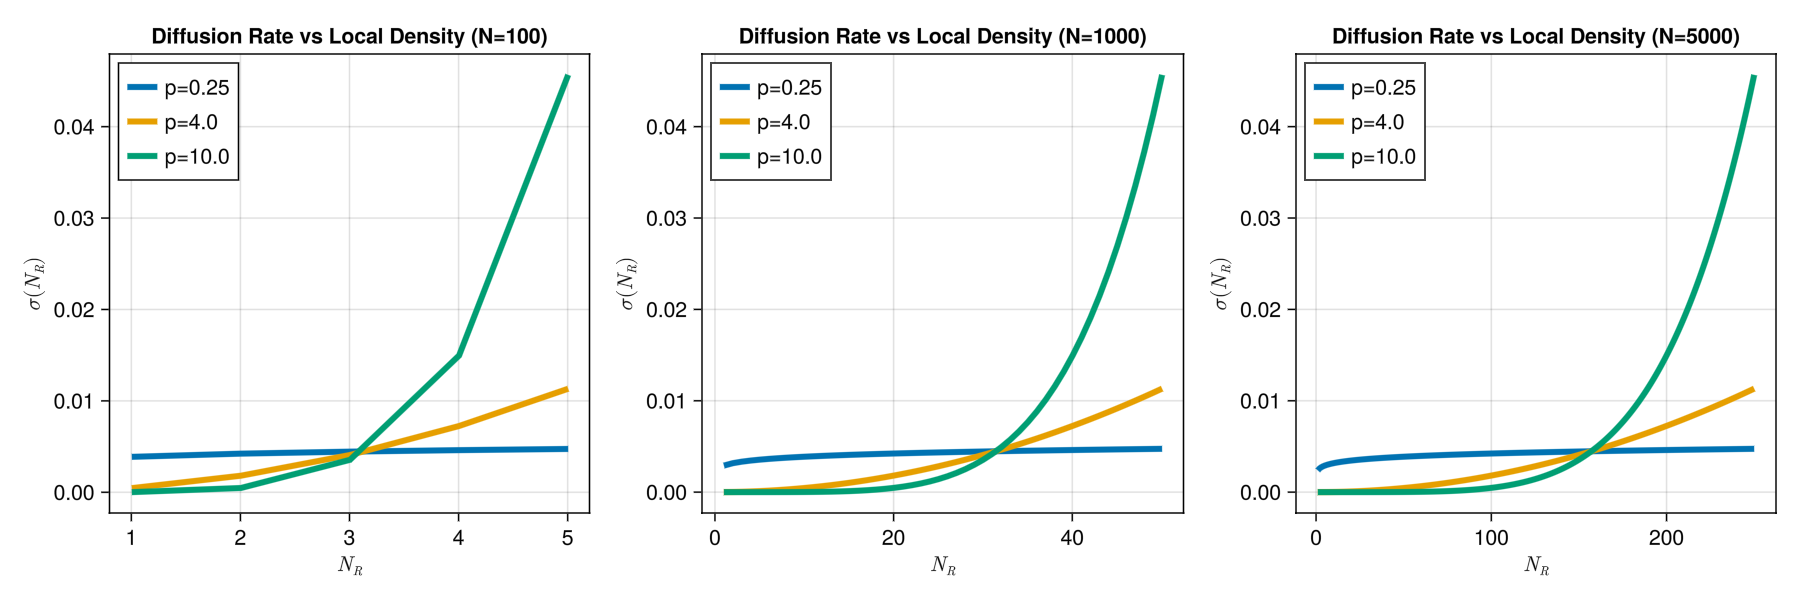
\includegraphics[width=1.0\linewidth]{img/diffusion_rates.png}
    \caption{Diffusion rate of an organism based on the number of organisms within distance $R$ for $N=100$, $N=1000$, $N=5000$ and $p=0.25$, $p=4$, $p=10$ and $D_0 = 0.001$. Note that while the shape of the curves is the same, the number of organisms that can be within the radius to reach a certain diffusion rate increases with the total number of organisms.}
\end{figure}

\subsection{A Single Organism}
Before moving on to the simulations, the diffusion of a single organism in space will be analysed.

To do this, we consider a simple environment with only a single organism and a constant diffusion term. 
This can be recovered from the density-dependent diffusion rate by setting $p=0$.
For simplicity, it will be assumed that the environment is infinite, as opposed to the torus used in the simulations.\\
The walker position will change similiarly to before, but with a constant diffusion term
\begin{align}
    & x(t + dt) = x(t) + \sqrt{2D dt} u_x \label{single_x}\\
    & y(t + dt) = y(t) + \sqrt{2D dt} u_y
\end{align}
where $u_x, u_y$ are independent random numbers $\sim \mathcal{N}(0,1)$.\\
Let's consider the increments $dx(t+dt) = x(t + dt) - x(t)$.
Then 
\begin{equation*}
    x(t) = \sum_{\tau = 0}^{t/dt} dx(\tau) + x(0),
\end{equation*}
that is, the position of $x$ at time $t$ can be described by adding up the increments.
From Eq. \ref{single_x}, we can see that the increments are normally distributed with variance $2D dt$.
The distribution of the displacements $x(t) - x(0)$ is therefore a sum of normally distributed random variables, thus being again normally distributed with the variance being the sum of the variances 
\begin{equation*}
    x(t) - x(0) \sim \mathcal{N}(0,\sum 2D dt) =  \mathcal{N}(0,2Dt).
\end{equation*}
To make the following equations clearer, we will use $\tilde{x}(t) = x(t)-x(0)$ and $\tilde{y}(t) = y(t)-y(0)$ .
Using this, we calculate the mean squared displacement 
\begin{equation*}
    MSD(t) = \langle \tilde{x}^2(t) +\tilde{y}^2(t) \rangle = \langle \tilde{x}^2(t)\rangle + \langle\tilde{y}^2(t) \rangle.
\end{equation*}
Again we focus on the term involving $x$.
\begin{align*}
    \langle \tilde{x}^2(t)\rangle = \int_{-\infty}^{\infty} \tilde{x}^2 p(\tilde{x},t)d\tilde{x} = \int_{-\infty}^{\infty} \tilde{x}^2 \frac{1}{\sqrt{4\pi Dt}} e^{-\frac{\tilde{x}^2}{4Dt}}d\tilde{x}
\end{align*}
Solving this integral requires a few steps, that will be only briefly mentioned. 
First, we do a variable transformation by setting $u = \frac{\tilde{x}}{\sqrt{4Dt}}$. 
The integral then becomes
\begin{equation*}
    \frac{4Dt}{\sqrt{\pi}}\int_{-\infty}^{\infty} u^2  e^{-u^2}du.
\end{equation*}
This integral can be solved by partial integration and is equal to $\sqrt{\pi}/2$.
Thus, the final result is 
\begin{equation*}
    \langle \tilde{x}^2(t)\rangle = 2Dt.
\end{equation*}
For $\langle \tilde{y}^2(t)\rangle$, we get the exact same result, and the mean squared displacement is therefore
\begin{equation*}
    MSD(t) = \langle \tilde{x}^2(t)\rangle + \langle \tilde{y}^2(t)\rangle  = 4Dt.
\end{equation*}
The average absolute distance of the organism from the initial position therefore grows with the square root of time.



\subsection{Stability Analysis}
Assuming that the population is large enough, we can approximate the dynamics with a continuous density equation given by
\begin{equation}
    \frac{\partial\rho(\vec{r},t)}{\partial t} = \nabla^2[D(\rho_R)\rho(\vec{r},t)],
\end{equation}
where $\rho(\vec{r},t)$ now describes the particle density at point $\vec{r}$ and time $t$ and
\begin{equation}
    D(\rho_R) = D_0 \left(\frac{\int_{R} \rho(\vec{r}',t)d\vec{r}'}{\pi R^2 \tilde{\rho}}\right)^p.
\end{equation}
The integral is taken over a disk of radius $R$ centered at $\vec{r}$. 
We will write the argument $\rho_R = \frac{\int_{R} \rho(\vec{r}',t)d\vec{r}'}{\pi R^2}$, which will make the subsequent analysis easier, because the function $D(\rho)=D_0 (\rho/\tilde{\rho})^p$ is simpler.

Following \cite{lopezMacroscopicDescriptionParticle2006}, we do a linear stability analysis to find under which conditions a uniform density is stable. 
A small perturbation of the uniform density $\rho_0$ will be written as $\rho_0 + \epsilon \Psi$, giving
\begin{align}
    \frac{\partial[\rho_0 + \epsilon \Psi](\vec{r},t)}{\partial t} &= \nabla^2\left[D\left(\frac{\int_{R} [\rho_0+\epsilon \Psi](\vec{r}',t)d\vec{r}'}{\pi R^2}\right)[\rho_0+\epsilon \Psi](\vec{r},t)\right]\\
    &= \nabla^2\left[D\left(\rho_0+\frac{\epsilon\int_{R} \Psi(\vec{r}',t)d\vec{r}'}{\pi R^2}\right)[\rho_0+\epsilon \Psi](\vec{r},t)\right] \label{stability1}
\end{align}
Expanding $D$ in $\rho_0$, we get 
\begin{equation}
    D(\rho_0+\epsilon \Psi_R) = D(\rho_0) + \epsilon \Psi_R D'(\rho_0) + \mathcal{O}(\epsilon^2),
\end{equation}
which we plug into Eq. (\ref{stability1}) to get

\begin{equation}
\nabla^2\left[\rho_0 D(\rho_0) + \rho_0\epsilon \Psi_R D'(\rho_0)+ D(\rho_0)\epsilon \Psi + \epsilon^2 \rho_0 \Psi_R D'(\rho_0) \Psi\right].
\end{equation}
The first term is $0$, since the density is uniform and we discard the last term because it is in $\mathcal{O}(\epsilon^2)$, leaving us with
\begin{equation}
    \frac{\partial \Psi(\vec{r},t)}{\partial t} = \nabla^2\left[ \rho_0  D'(\rho_0)\Psi_R(\vec{r},t)+ D(\rho_0) \Psi(\vec{r},t) \right].
\end{equation}
Assuming a harmonic perturbation $\Psi(\vec{r}, t) = \Psi_0 e^{(\lambda t + i \vec{k} \cdot \vec{x})}$ and using Fourier analysis, $\lambda$ can be derived.
Depending on the sign of $\lambda$, the perturbations will either grow or decay over time.
From \cite{lopezMacroscopicDescriptionParticle2006}, we find that 
\begin{equation}
    \lambda(\vec{k}) = -D_0 k^2\left(1 + \frac{2pJ_1(kR)}{kR}\right),
\end{equation}
where $J_1$ is the first-order Bessel function.
The paper also states a critical value of $p\sim 7.6$, for which $\lambda $ becomes positive, though there is no discussion about the value of $k$ for which this is attained. 
That means that the onset of pattern formation occurs around $p_c \sim 7.6$ and independent of $D_0$.

\subsection{Radial Correlation Function}
The radial correlation function indicates the distribution of particles. 


\subsection{Simulation}
Numerical simulations of the system with density-dependent diffusion rates were implemented in the programming language julia.
To keep things managable, three population sizes are simulated, $N_1=100, N_2 = 1000, N_3 = 5000$.
For each population size, the simulation was run for a number of values of the parameters $p$ and $D_0$.
Based on the stability analysis, for $N_1$ and $N_2$, $40$ evenly spaced values between $5$ and $10$ were simulated for the parameter $p$ and $10$ values were used for the largest population $N_3$.
The parameter $D_0$ was simulated across a broader range, from $10^{-1}$ to $10^{-4}$ and for $N_1$ and $N_2$, $40$ logarithmically evenly spaced values were used, while for $N_3$ $10$ values were simulated as well.
For $N_3$, a smaller number of parameters was simulated because the computation time would be too high to simulate the same number of particles as in the other cases.
The initial positions of the particles was drawn from a uniform distribution on a square of sidelength 1.

To allow patterns to form, the simulation was be run for $n=2000$ steps. 
At the end of the simulation, the radial calculation is calculated and its mean deviation from $1$ recorded. 
The MSD between the radial distribution function and $g(r) \equiv 1$ was recorded at the end of each simuation and recorded on a heatmap.

\section{Results} 
The results of the simulations for the three different population sizes will be presented here.
For each population size, 24 parameter combinations were tested.





\subsection{Medium Population}
The results for $N=1000$ will be presented first, because they contain the least amount of noise.
For given parameters, the spatial distribution generally falls in one of two categories, either being slightly overdispersed or clumped. 

Clumped patterns form when the baseline diffusion rate $D_0$ is small and the exponent $p$ in the diffusion kernel is high. 
In the simulations, clumped patterns could be observed for $D_0 \in \{0.01, 0.001, 0.0001\}$ and $p\in\{8, 10\}$.
One of the least noisy examples of clumped spatial patterns can be seen in Fig. \ref{rp68}.

If the baseline diffusion rate $D_0$ is high, then no clumped patterns form for all tested values of $p$. 
% resultplot 51 - 74 
\begin{figure}
    \label{rp68}
    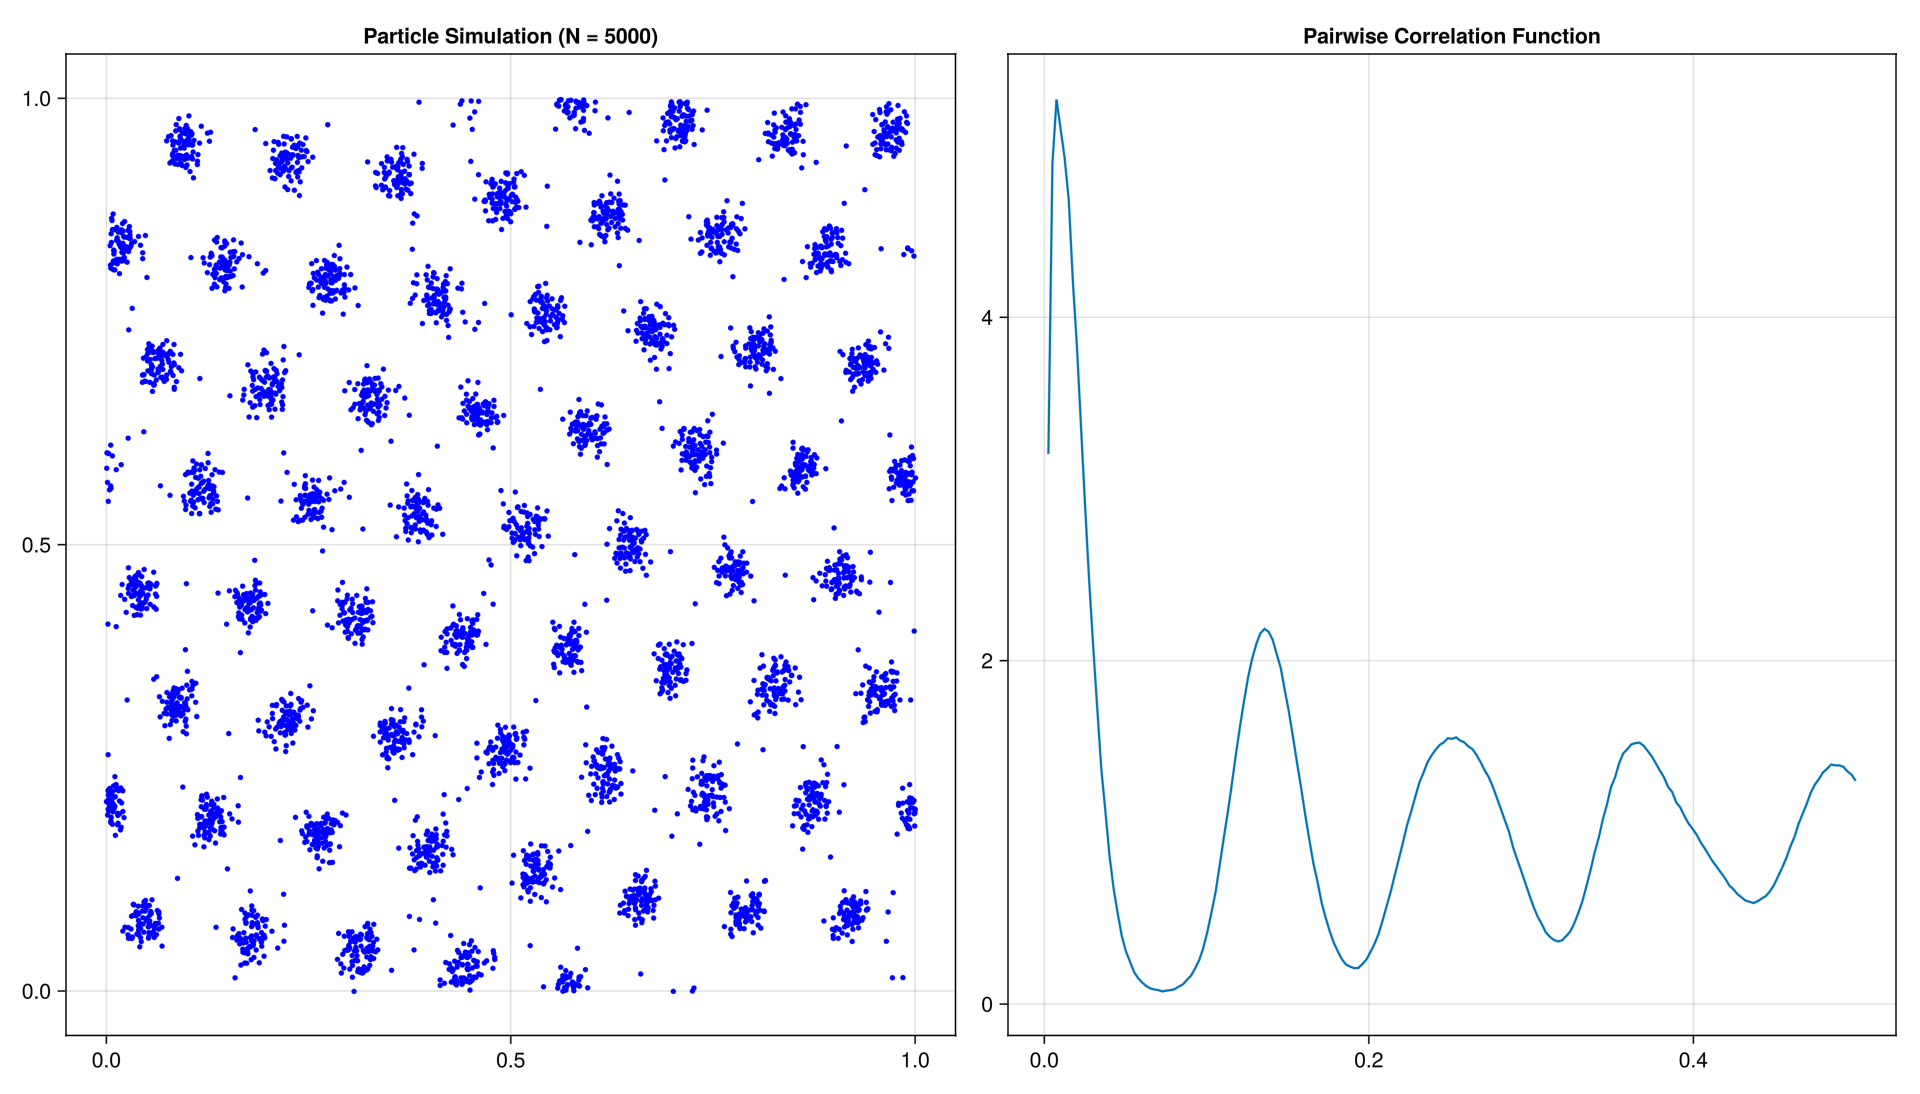
\includegraphics[width=1.0\linewidth]{img/rp68_N5000_D01_p8.png}
    \caption{Results of the simulation with $N=5000$, $p=8$, $D_0=0.01$.}
\end{figure}

\subsection{Medium Population}

For $N=1000$, the shift seems to occur around $p=6$, where some clumped patterns can be seen 
\section{Discussion}
\printbibliography
\end{document}